%\documentclass[12pt,letterpaper,titlepage]{article}
\documentclass[11pt,letterpaper, one-sided]{article}
\usepackage[top=2.5cm, bottom=2.5cm, left=2.5cm, right=2.5cm]{geometry}
\usepackage{changepage}
\usepackage{amsmath}
\usepackage{amssymb}
\usepackage{graphicx}

% Edit these as appropriate
\newcommand\course{Database Design and Implementation}
\newcommand\semester{Spring 2014}     % <-- current semester
\newcommand\yourname{Vijay Kumar Pasikanti} % <-- y	our name
\newcommand\testname{Mid-Term Project Report}
\newcommand{\ttt}[1]{\textit{#1}}

\newenvironment{answer}[1]{
  \subsection*	{#1}
}

\newenvironment{subanswer}[1]{
  \subsubsection*{#1}
}

\begin{document}
\title{\large{\textbf{\Large\course}\\ \semester \\\textbf{\testname}}}
\author{\textbf{Submitted by:} \\ \yourname, Ashish Jain\\\{vijaykp,ashishjain\}@cs.umass.edu}
\maketitle

\begin{answer}{Introduction:}
Graph data management systems have been receiving a lot of attention with the arrival of various social networks like Facebook, Twitter, Google+ etc. All these social networks have their data stored in some or the other form of graph with billions of nodes. Graph databases processing relations between nodes effectively and their efficiency on running graph queries have made relational databases not a preferred choice for these kind of applications. Connectivity and adjacency between nodes in these networks can reveal interesting properties if one has to analyze them. Clustering is one of the graph properties which when applied to social networks produces communities which are tightly connected within themselves. \\\\
The goal of the project is to present a comprehensive study of performance of various graph databases on community detection algorithms. The next few sections of the report talk about the design, implementation and evaluation.
\end{answer}

\begin{answer}{Design}
	\begin{subanswer}{Data Generation:}
	Data Generation: Our main goal is to compute benchmark of various graph databases using clustering algorithm on social network data. Therefore we simulated generation of community structure in our data using Networkx. First, we generated single communities with high clustering coefficient and thereafter we combined them to form a complete social network graph. The edges between the communities are added using internal probability based function that makes sure that each of the individual communities maintains their identity.\\
	\\
	Following is the sample of data generated with three communities with a total 90 users.
	\begin{center}
		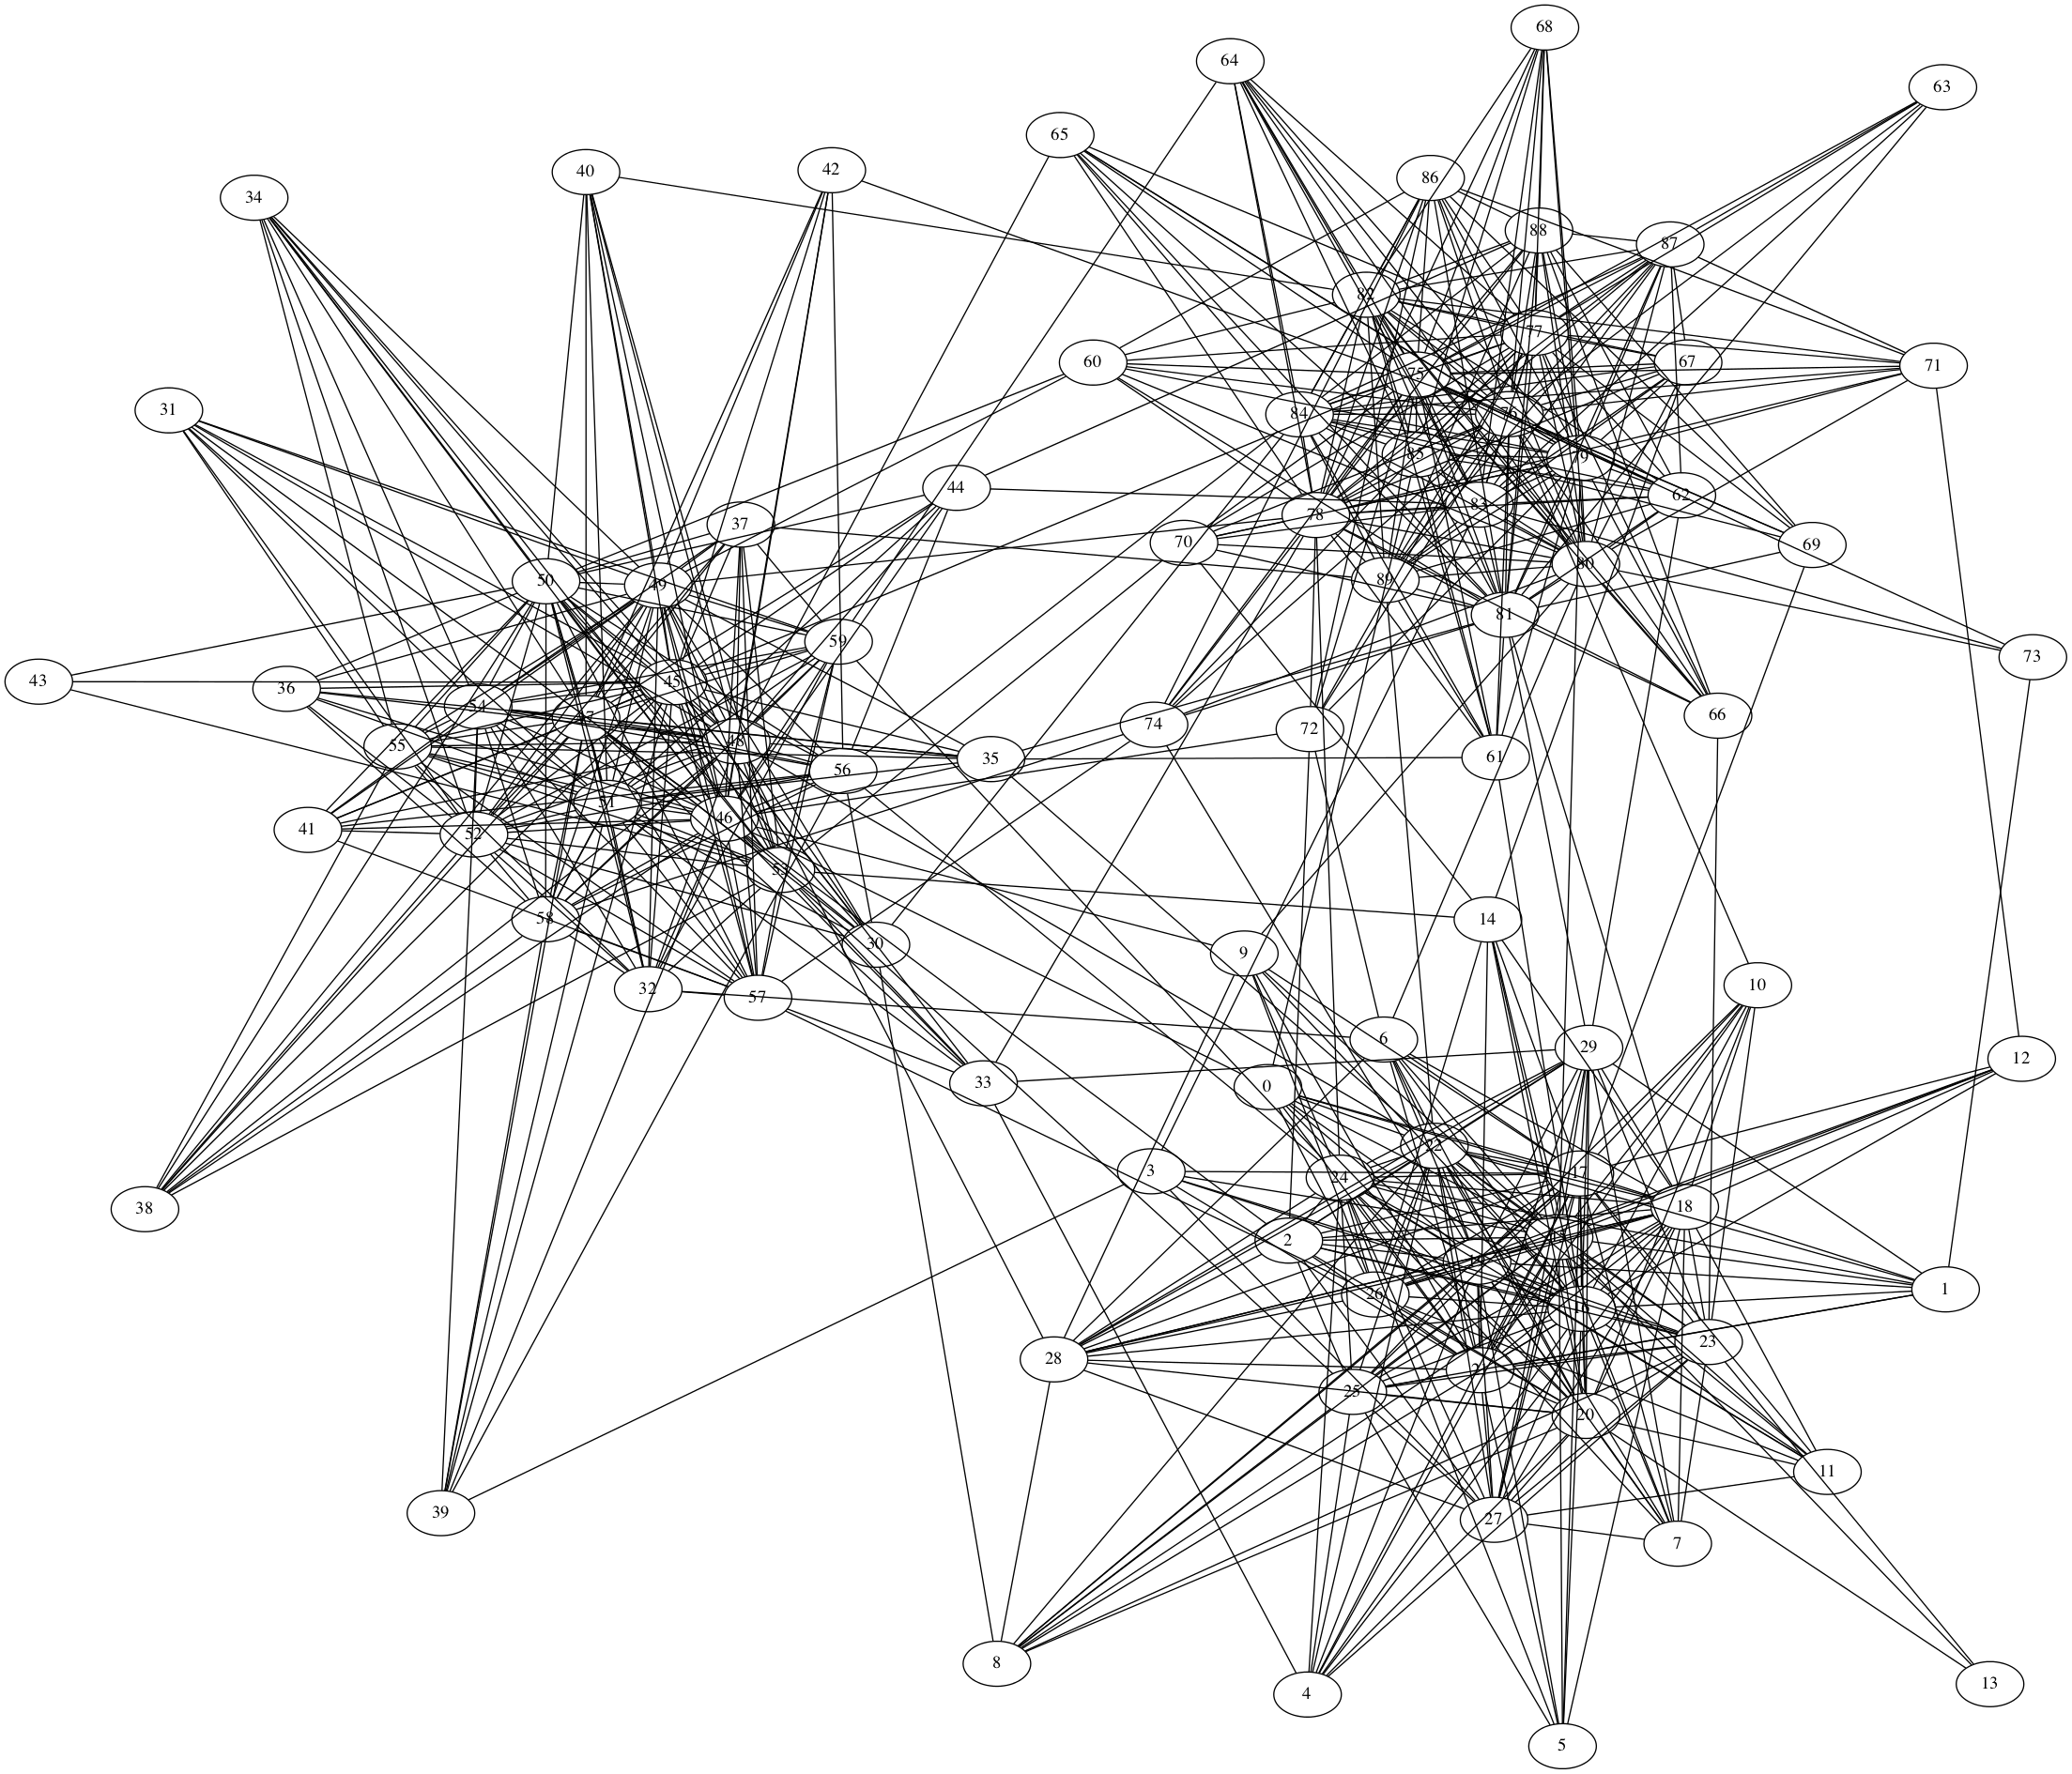
\includegraphics[scale=.15]{90_nodes.png}
	\end{center}
	\end{subanswer}

	\begin{subanswer}{Algorithm:}
		We followed the hierarchical clustering approach with two passes over the entire database. Since we generated synthetic data with no distinctive properties for each vertex, we assorted to adjacency based measure like neighborhood of a node for first pass of graph clustering. We also used clustering coefficient for computing the final clusters from the first pass of clusters. Neighbors for each node are retrieved from the database using the Neo4j internal query. 
		\\\\
		Neighbor similarity is computed using \textit{Jaccard index} which is defined for two sets of nodes A and B as
		$$ \rho(A, B) = \frac{|A| \cap |B|}{|A|\cup|B|} $$
		\\
		Since we are dealing with simulated data of social network, clustering coefficient is a preferable measure because clustering coefficient is a measure of the degree to which nodes in a graph tend to cluster together and in real-world networks, in particular social networks, nodes tend to create tightly knit groups by a relatively high density of ties. This measure is used in the second pass of clustering while combining bigger groups of nodes. 
		\\\\
		Clustering coefficient ($C$) is based on triplets of nodes. A triplet consists of three nodes that are connected by either two (open triplet) or three (closed triplet) undirected ties. A triangle consists of three closed triplets, one centred on each of the nodes. The clustering coefficient is the number of closed triplets (or 3 x triangles) over the total number of triplets (both open and closed). 
		$$C = \frac{3\times Number Of Triangles}{number Of Connected Triples Of Vertices} = \frac{Number Of Closed Triplets}{Number Of Connected Triples Of Vertices} $$
	\end{subanswer}
	\begin{subanswer}{Implementation:}
		\begin{enumerate}
			\item
			We have implemented breadth first traversal to traverse the entire graph database, node by node. In first pass of the clustering algorithm each node is treated as an individual cluster. 
			\item
			We compute Jaccard Index based on number of neighbors each node share. If a node is merged into a cluster it will become part of it and no more appear as a single node cluster. We have set the threshold of Jaccard Index very high in order to merge two clusters. Therefore, we got highly connected clusters based on the similarity of neighbors two nodes share.
			\item
			After doing first pass clustering, we merge the fragmented clusters to detect the entire community structure. Clustering coefficient is know to identify the close knit groups in real world networks like social network. Two clusters are combined when the clustering coefficient of the union of two subgraphs generated out of the nodes in two clusters, is above certain threshold value. We tuned this threshold value based on our observation of clusters formed. Currently, we are finding out the best possible cluster combination in our algorithm which is giving polynomial time complexity, hence high running time.
		\end{enumerate}
	\end{subanswer}
\end{answer}

\begin{answer}{Evaluation:}
	We generated small datasets of size 300, 900, 3000 and 6000 nodes in order to check robustness of our clustering algorithm, as well as verifying the correctness of our work. We used neo4j graph database for storing the synthetic graph data and it is accessed through a python package \textit{py2neo}.  Our programs were run on Amazon EC2 instance running a VM with Ubuntu with 7.5 GB RAM and 2 vCPUs.
	\\\\
	To verify the robustness of our clustering algorithm, we generated three communities of 100 nodes each. Then we combined them to form a graph of 300 nodes along with addition of enough edges between the groups. On clustering this graph, we get following as the clusters:
	\\\\
	Clusters after final pass
	\begingroup
	\fontsize{10pt}{12pt}
	\begin{verbatim}
	['4', '5', '8', '9', '12', '13', '15', '16', '17', '18', '19', '21', '22', '23', '25', 
	'26', '27', '28', '31', '1', '40', '41', '42', '43', '44', '45', '46', '47', '48', '50', 
	'51', '52', '54', '55', '56', '57', '58', '59', '60', '61', '62', '63', '66', '67', 
	'73', '76', '77', '80', '86', '88', '96', '97', '98', '0', '2', '3', '6', '7', '10',
	'11', '14', '20', '49', '53', '64', '65', '68', '69', '70', '71', '72', '74', '75', 
	'78', '79', '81', '82', '83', '84', '85', '87', '90', '91', '92', '93', '94', '95', 
	'99', '89', '37', '39', '24', '29', '30', '32', '33', '34', '35', '36', '38' ]
	Nodes:100
	['232', '224', '229', '230', '231', '233', '234', '238', '217', '236', '235', '227', 
	'226', '204', '205', '208', '209', '212', '213', '215', '216', '218', '219', '221', 
	'222', '223', '225', '228', '240', '257', '244', '202', '263', '270', '289', '252', 
	'214', '200', '201', '203', '206', '207', '210', '211', '220', '241', '242', '243', 
	'245', '246', '247', '248', '249', '250', '251', '253', '254', '255', '256', '258', 
	'259', '260', '261', '262', '264', '265', '266', '267', '268', '269', '271', '272', 
	'273', '274', '275', '276', '278', '279', '280', '281', '282', '283', '284', '285', 
	'286', '287', '288', '290', '291', '292', '293', '294', '295', '296', '297', '298', 
	'299', '277', '237', '239']
	Nodes:100
	['131', '139', '115', '134', '128', '116', '108', '112', '121', '101', '109', '113', 
	'117', '118', '119', '122', '123', '125', '126', '127', '105', '100', '185', '155', 
	'191', '104', '194', '164', '163', '199', '196', '103', '141', '106', '107', '110', 
	'111', '114', '120', '140', '142', '143', '144', '145', '146', '148', '149', '150', 
	'152', '153', '156', '157', '158', '159', '160', '165', '166', '167', '168', '169', 
	'173', '181', '182', '187', '188', '189', '190', '192', '195', '197', '198', '147', 
	'151', '154', '161', '162', '170', '171', '172', '174', '175', '176', '177', '178', 
	'179', '180', '183', '184', '186', '193', '102', '137', '132', '133', '136', '124', 
	'129', '130', '135', '138']
	Nodes:100
	\end{verbatim}
	\endgroup
	\noindent
	Except few outliers, we are getting nearly perfect clustering with nodes numbered 1-100, 101-200 and 201-300 lying in the same cluster.
	\begin{subanswer}{Results:}
		The following plot shows the performance of clustering of synthetic graph datasets on Neo4j database. We can clearly see the exponential increase in the time of execution as the number of nodes grow in the graph.
			\begin{center}
				\includegraphics[scale=.4]{plot1.pdf}
			\end{center}
	\end{subanswer}

\end{answer}
\begin{answer}{Future work}
	\begin{enumerate}
	\item
	Integrate the clustering algorithm with other graph databases and compare their performance with neo4j.
	\item
	Use performance metrics collection software, like Ganglia, to collect CPU, memory utilization stats during the algorithm execution.
	\item
	Large dataset of about million nodes needs to be generated to compare clustering performance in terms of time and memory requirements. Ours would be the first work performing the benchmark study of this task. In earlier works, algorithms like shortest path traversal and page rank were compared.
	\item
	We need to improve upon the second pass of the clustering algorithm to reduce the total execution time of the algorithm.
	\end{enumerate}
\end{answer}
\end{document}          
